\documentclass[main.tex]{subfiles}
\begin{document}
\section{Algorithm}

\begin{figure}[htpb]
  \centering
  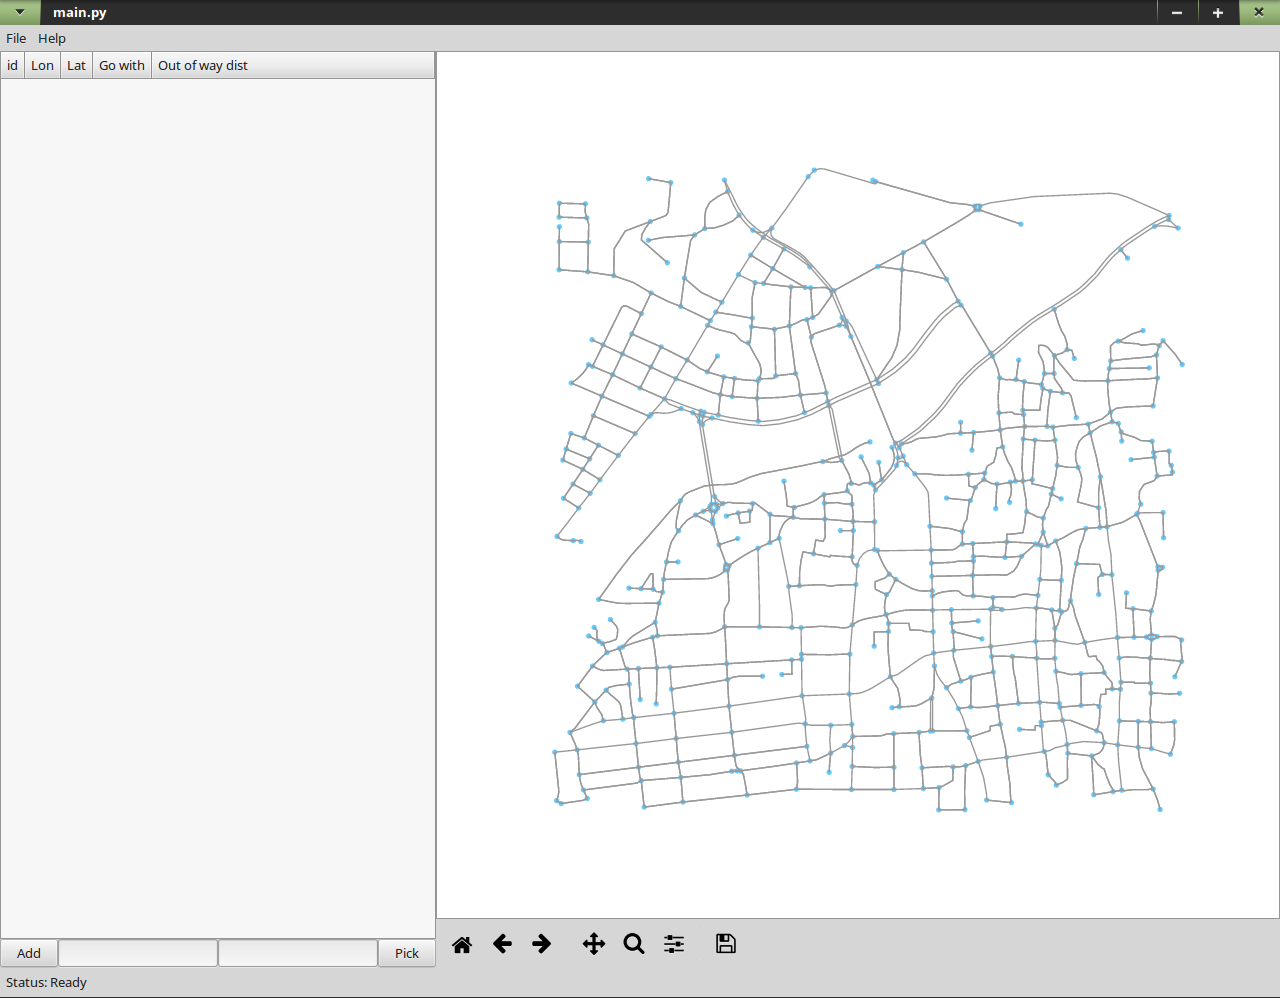
\includegraphics[width=0.8\linewidth]{scr_1.png}
  \caption{Initial map}
  \label{fig:scr1}
\end{figure}

Initially, the road map is loaded. The downloaded data representes the roads as
a sequence of line segments. These are all collapsed to to create a network
graph from the actual road network. This forms a simplified logical view of the
problem from the given physical road layout.


\begin{figure}[htpb]
  \centering
  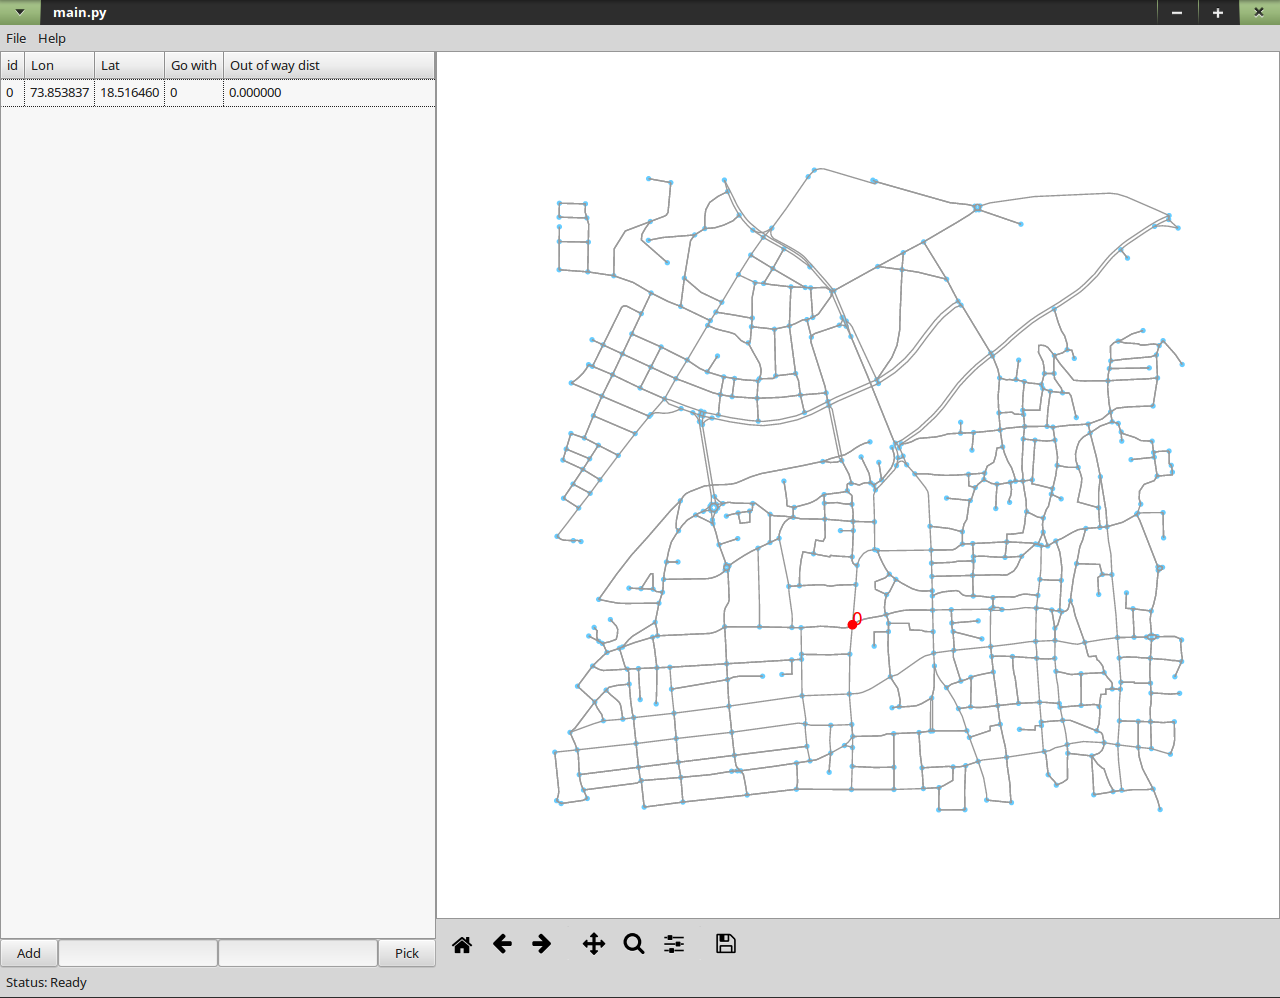
\includegraphics[width=0.8\linewidth]{scr_2.png}
  \caption{Common point placed}
  \label{fig:scr2}
\end{figure}

When a location on the map is picked, the nearest node (intersection) is
selected, so as to obtain a node in the simplified graph. The first node picked
is the common destination for all drivers.

One improvement can be to create a new node by splitting the graph at the edge
nearest to the picked location, which will be technically the destination.
However, for a dense city, the nearest intersection can be used as a good
approximation. This gives more possiblilities for paths between the starting
points of any drivers (and we can assume that everyone is capable of walking to
the nearest intersection)


\begin{figure}[htpb]
  \centering
  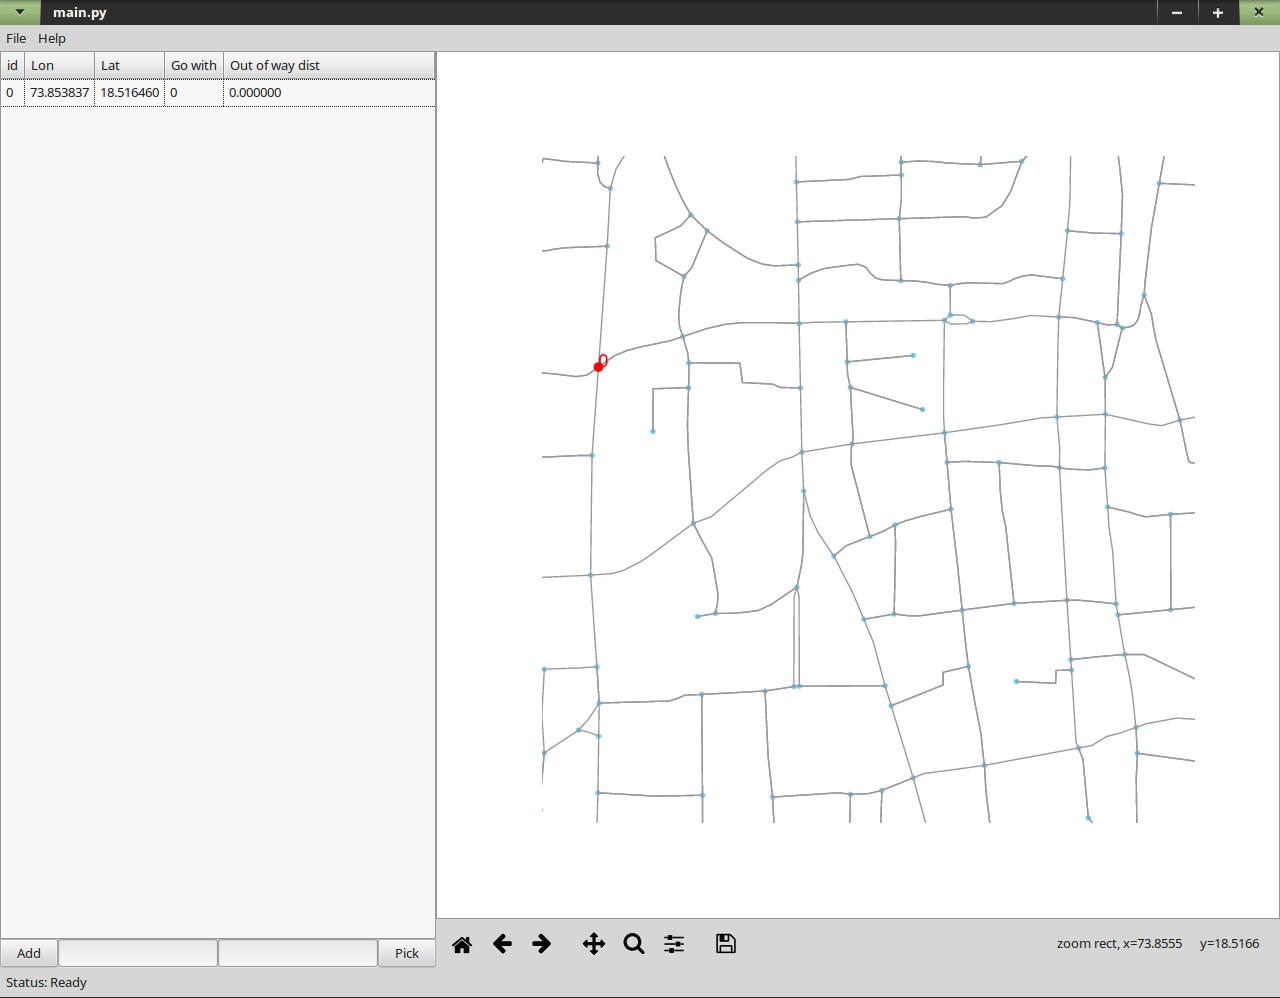
\includegraphics[width=0.8\linewidth]{scr_3.png}
  \caption{Zoomed view at common point}
  \label{fig:scr3}
\end{figure}


\begin{figure}[htpb]
  \centering
  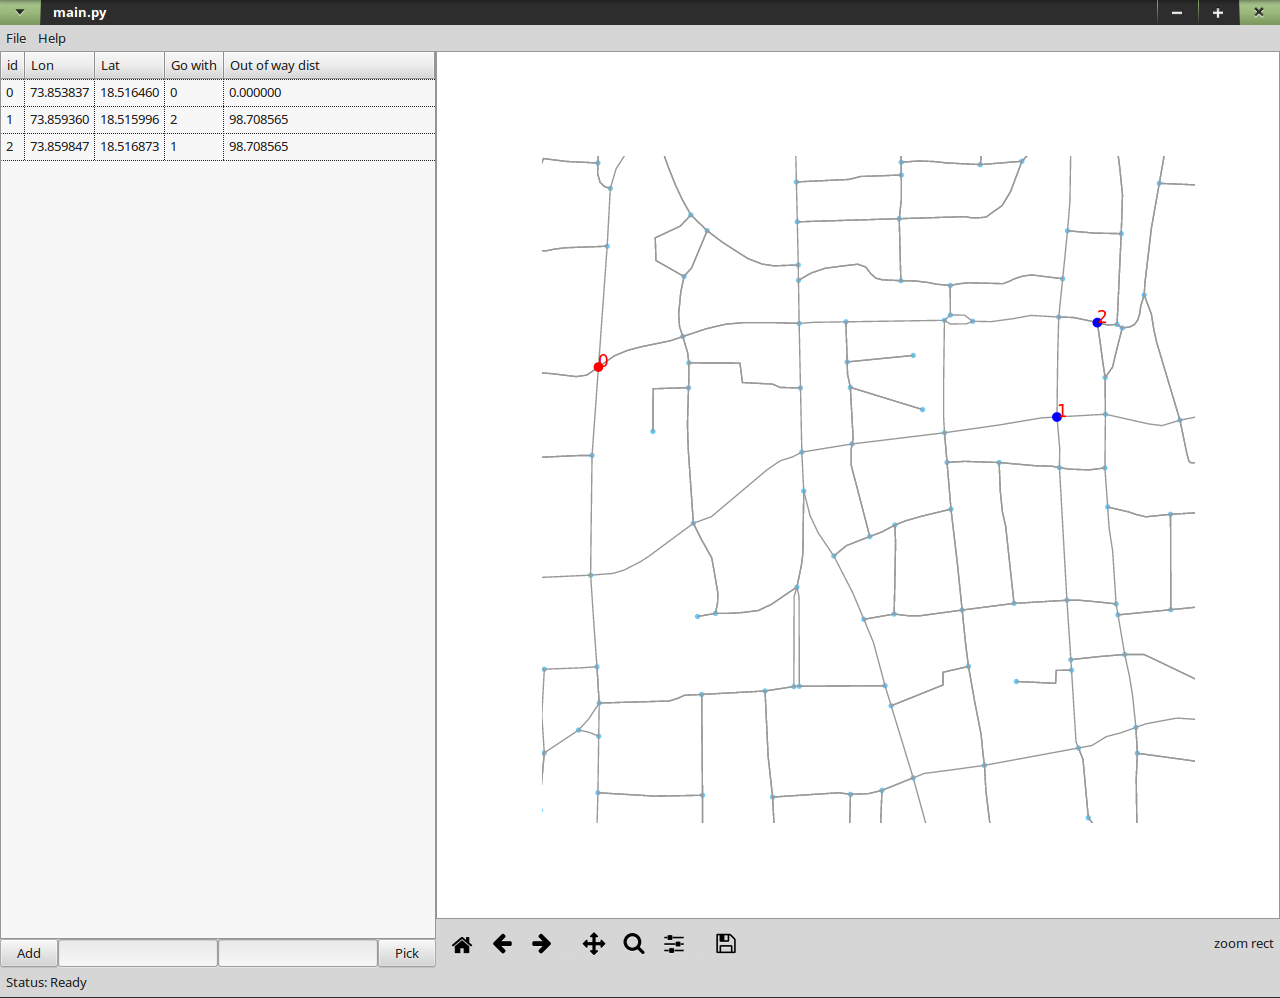
\includegraphics[width=0.8\linewidth]{scr_4.png}
  \caption{First two drivers placed}
  \label{fig:scr4}
\end{figure}

Once the first two drivers are placed, the algorithm calculates pairwise
shortest distance between each driver and from each driver to the destination.
This further simplifies the graph used to represent the problem, as the actual
or logical road layout is no longer required.

These shortest distances form a complete directed (distance may differ due to
road features such as one-ways) graph which captures the required details of the
actual road network.

\begin{figure}[htpb]
  \centering
  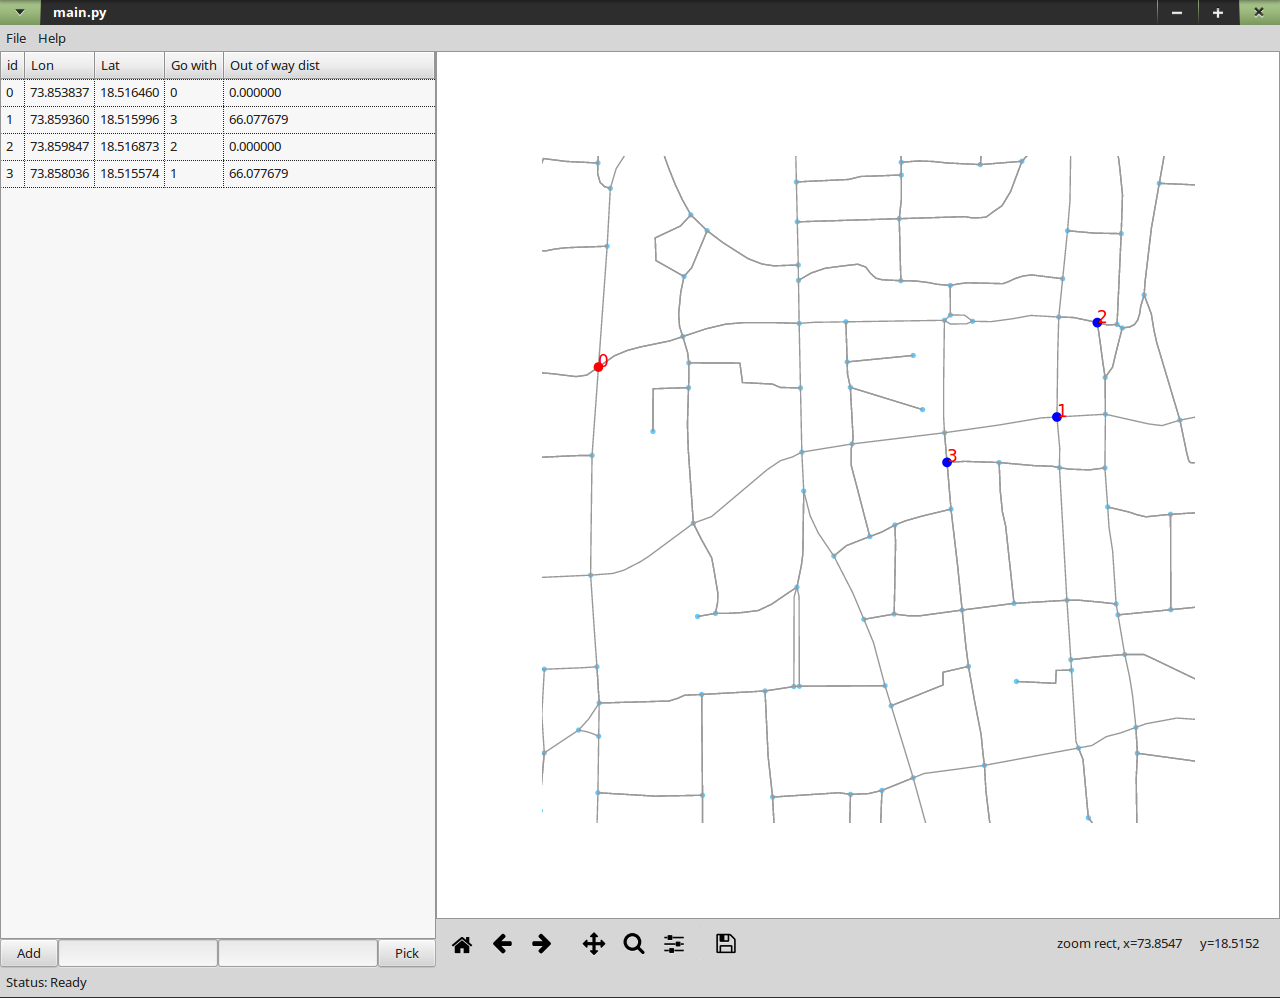
\includegraphics[width=\linewidth]{scr_5.png}
  \caption{Final matching with three drivers}
  \label{fig:scr5}
\end{figure}

\begin{figure}[htpb]
  \centering
  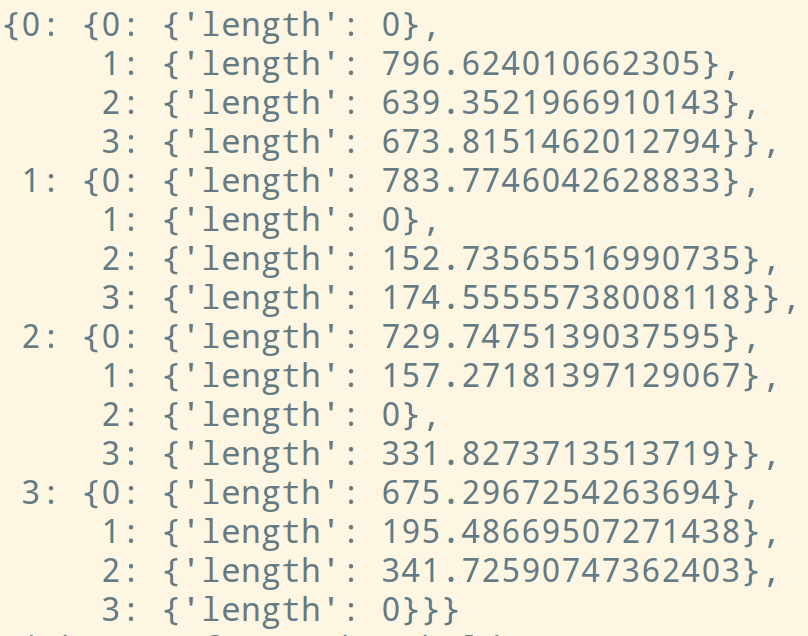
\includegraphics[width=\linewidth]{pairwise_1.png}
  \caption{Pairwise distances}
  \label{fig:p1}
\end{figure}

\begin{figure}[htpb]
  \centering
  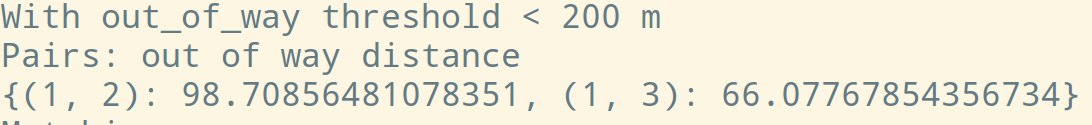
\includegraphics[width=\linewidth]{compatibility_1.png}
  \caption{Compatible pairs and extra distance}
  \label{fig:p1}
\end{figure}
Next, feasible pairs of drivers are chosen based on a threshold limit that
drivers are willing to go out of their way to pick up another person. The
algorithm is as:

\begin{verbatim}
For every pair Vi, Vj of distinct nodes:
      extra_dist_1 = abs(dist(Vi->Vj) + dist(Vj->dest) - dist(Vi->Dest))
      extra_dist_2 = abs(dist(Vj->Vi) + dist(Vi->dest) - dist(Vj->Dest))
      extra_dist = min(extra_dist_1, extra_dist_2)
      if extra_dist < threshold:
          Add (Vi--Vj) to a undirected graph G with edge weight = extra_dist
\end{verbatim}

This constructs a new undirected graph G, which connects compatible pairs with
an edge. The edge weigths show the extra distance that one of the person has to
travel to pick up the other.

Since our assumption is based on only two drivers pairing up to share a ride, we
can now chose pairs from this graph using maximum matching.
Out of all possible maximum matchings on graph G, we pick the one that minimizes
sum of edge weights.


\end{document}
